\subsection{Đề 2}
\caulc
\begin{ex}%[Câu 1]%[2D1N5-1]
	Đồ thị của hàm số nào dưới đây có dạng như đường cong trong hình bên?
	\begin{center}
		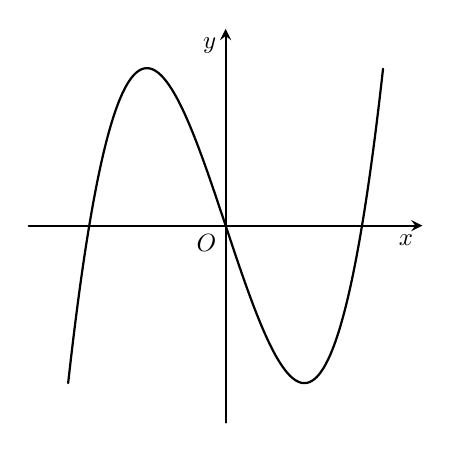
\begin{tikzpicture}[line join=round, line cap=round,>=stealth,thick]
			\tikzset{every node/.style={scale=0.9}}
			\draw[->] (-2.5,0)--(2.5,0) node[below left] {$x$};
			\draw[->] (0,-2.5)--(0,2.5) node[below left] {$y$};
			\draw (0,0) node [below left] {$O$};
			\begin{scope}
				\clip (-2.5,-2.5) rectangle (2.5,2.5);
				\draw[samples=200,domain=-2:2,smooth,variable=\x] plot (\x,{1*((\x)^3)+0*((\x)^2)+-3*(\x)+0});
			\end{scope}
		\end{tikzpicture}	
	\end{center}
	\choice
	{\True $y=x^3-3x$ }
	{$y=-x^3+3x$ }
	{$y=x^2-2x$}
	{$y=-2x^2+3$}
	\loigiai{
		Đường cong có dạng của đồ thị hàm số bậc ba với hệ số $a>0$ nên chỉ có hàm số $y=x^3-3x$ thỏa yêu cầu bài toán.
	}
\end{ex}
\begin{ex}%[Câu 2]%[2D1H5-1]
	Hàm số nào dưới đây có bảng biến thiên như hình bên dưới?
	\begin{center}
		
\begin{tikzpicture}
			\tkzTabInit[espcl=3,lgt=1.5]
			{$x$/0.7,$y'$/0.7,$y$/2.1}
			{$-\infty$,$5$,$+\infty$}
			\tkzTabLine{,-,d,-,}
			\tkzTabVar{+/$1$,-D+/$-\infty$/$+\infty$,-/$1$}
		\end{tikzpicture}
	\end{center}
	\choice
	{$y=\dfrac{x-7}{x-5}$}
	{$y=\dfrac{x-5}{x-1}$}
	{$y=\dfrac{5x}{x-1}$}
	{\True $y=\dfrac{x-3}{x-5}$}
	\loigiai{
		Theo bảng biến thiên ta có\\
		Tiệm cận đứng có phương trình $x=5$, tiệm cận ngang có phương trình $y=1$ và $y'<0 ~ \forall x \in \mathbb{R}$ nên ta chọn hàm số $y=\dfrac{x-3}{x-5}$.
	}
\end{ex}
\begin{ex}%[Câu 3]%[2D1H5-2]
	Cho hàm số $y=f(x)$ xác định, liên tục trên $\mathbb{R}$ và có đồ thị như hình bên.
	\begin{center}
		\begin{tikzpicture}[line join=round, line cap=round,>=stealth,thick]
			\tikzset{every node/.style={scale=0.9}}
			\draw[->] (-2.5,0)--(2,0) node[below] {$x$};
			\draw[->] (0,-1.1)--(0,3.1) node[below left] {$y$};
			\draw (0,0) node [below left] {$O$};
			\foreach \x/\nx in {1/1}
			\draw[thin] (\x,1pt)--(\x,-1pt) node [below] {$\nx$};
			\foreach \y/\ny in {1/1}
			\draw[thin] (1pt,\y)--(-1pt,\y) node [left] {$\ny$};
			\begin{scope}
				\clip (-2.5,-1) rectangle (1.5,3);
				\draw[samples=200,domain=-2.5:2.5,smooth,variable=\x] plot (\x,{3^(\x)});
			\end{scope}
		\end{tikzpicture}
	\end{center}
	Đồ thị nào dưới đây là đồ thị của hàm số $y=f(x)+1$?
	\choice
	{\begin{tikzpicture}[line join=round, line cap=round,>=stealth,thick]
			\tikzset{every node/.style={scale=0.9}}
			\draw[->] (-2.5,0)--(2,0) node[below] {$x$};
			\draw[->] (0,-1.1)--(0,3.1) node[below left] {$y$};
			\draw (0,0) node [below left] {$O$};
			\foreach \x/\nx in {1/1}
			\draw[thin] (\x,1pt)--(\x,-1pt) node [below] {$\nx$};
			\foreach \y/\ny in {1/1}
			\draw[thin] (1pt,\y)--(-1pt,\y) node [left] {$\ny$};
			\begin{scope}
				\clip (-2.5,-1) rectangle (1.5,3);
				\draw[samples=200,domain=-2.5:2.5,smooth,variable=\x] plot (\x,{3^(\x)});
			\end{scope}
	\end{tikzpicture}}
	{\True \begin{tikzpicture}[line join=round, line cap=round,>=stealth,thick]
			\tikzset{every node/.style={scale=0.9}}
			\draw[->] (-2.5,0)--(2,0) node[below] {$x$};
			\draw[->] (0,-1.1)--(0,3.1) node[below left] {$y$};
			\draw (0,0) node [below left] {$O$};
			\foreach \x/\nx in {1/1}
			\draw[thin] (\x,1pt)--(\x,-1pt) node [below] {$\nx$};
			\foreach \y/\ny in {1/1, 2/2}
			\draw[thin] (1pt,\y)--(-1pt,\y) node [left] {$\ny$};
			\begin{scope}
				\clip (-2.5,-1) rectangle (1.5,3);
				\draw[samples=200,domain=-2.5:2.5,smooth,variable=\x] plot (\x,{3^(\x)+1});
			\end{scope}
	\end{tikzpicture}}
	{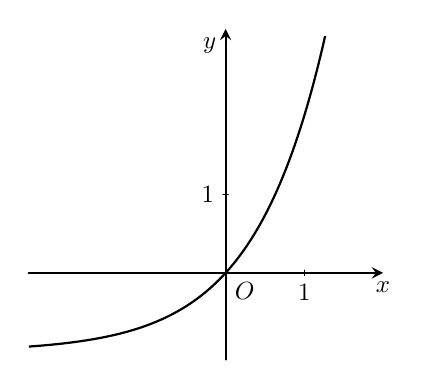
\begin{tikzpicture}[line join=round, line cap=round,>=stealth,thick]
			\tikzset{every node/.style={scale=0.9}}
			\draw[->] (-2.5,0)--(2,0) node[below] {$x$};
			\draw[->] (0,-1.1)--(0,3.1) node[below left] {$y$};
			\draw (0,0) node [below right] {$O$};
			\foreach \x/\nx in {1/1}
			\draw[thin] (\x,1pt)--(\x,-1pt) node [below] {$\nx$};
			\foreach \y/\ny in {1/1}
			\draw[thin] (1pt,\y)--(-1pt,\y) node [left] {$\ny$};
			\begin{scope}
				\clip (-2.5,-1) rectangle (1.5,3);
				\draw[samples=200,domain=-2.5:2.5,smooth,variable=\x] plot (\x,{3^(\x)-1});
			\end{scope}
	\end{tikzpicture}}
	{\begin{tikzpicture}[line join=round, line cap=round,>=stealth,thick]
			\tikzset{every node/.style={scale=0.9}}
			\draw[->] (-2.5,0)--(2,0) node[below] {$x$};
			\draw[->] (0,-1.1)--(0,3.1) node[below left] {$y$};
			\draw (0,0) node [below left] {$O$};
			\foreach \x/\nx in {1/1}
			\draw[thin] (\x,1pt)--(\x,-1pt) node [below] {$\nx$};
			\foreach \y/\ny in {1/1, 2/2}
			\draw[thin] (1pt,\y)--(-1pt,\y) node [left] {$\ny$};
			\begin{scope}
				\clip (-2.5,-1) rectangle (1.5,3);
				\draw[samples=200,domain=-2.5:2.5,smooth,variable=\x] plot (\x,{3^(\x+0.7)});
			\end{scope}
	\end{tikzpicture}}
	\loigiai{
		Từ đồ thị hàm số $y=f(x)$ tìm đồ thị hàm số $y=f(x)+a$.\\
		Tịnh tiến đồ thị hàm số $y=f(x)$ lên phía trên (theo phương $Oy$) $a$ đơn vị nếu $a>0$.\\
		Hàm số $y=f(x)+1 \Rightarrow a=1>0$ nên ta được đồ thị hàm số cần tìm tịnh tiến đồ thị hàm số $y=f(x)$ lên phía trên (theo phương $Oy$) $1$ đơn vị.
	}
\end{ex}
\begin{ex}%[Câu 4]%[2D1H5-3]
	Cho hàm số bậc ba $y=f(x)$ có đồ thị là đường cong trong hình bên. Số nghiệm thực của phương trình $f(x)=-1$ là
	\begin{center}
		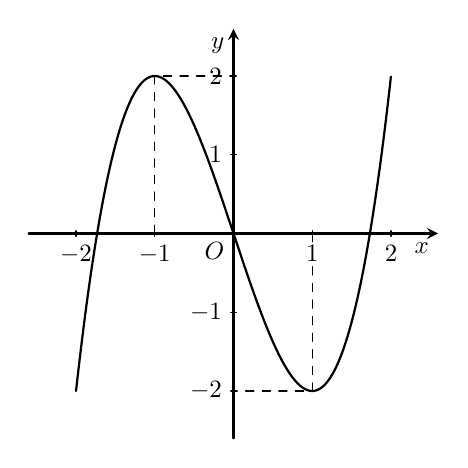
\begin{tikzpicture}[line join=round, line cap=round,>=stealth,thick]
			\tikzset{every node/.style={scale=0.9}}
			\draw[->] (-2.6,0)--(2.6,0) node[below left] {$x$};
			\draw[->] (0,-2.6)--(0,2.6) node[below left] {$y$};
			\draw (0,0) node [below left] {$O$};
			\foreach \x/\nx in {-2/-2,-1/-1,1/1,2/2}
			\draw[thin] (\x,1pt)--(\x,-1pt) node [below] {$\nx$};
			\foreach \y/\ny in {-2/-2,-1/-1,1/1,2/2}
			\draw[thin] (1pt,\y)--(-1pt,\y) node [left] {$\ny$};
			\draw[dashed,thin](-1,0)--(-1,2)--(0,2);
			\draw[dashed,thin](1,0)--(1,-2)--(0,-2);
			\begin{scope}
				\clip (-2.5,-2.5) rectangle (2.5,2.5);
				\draw[samples=200,domain=-2:2,smooth,variable=\x] plot (\x,{1*((\x)^3)+0*((\x)^2)+-3*(\x)+0});
			\end{scope}
		\end{tikzpicture}
	\end{center}
	\choice
	{\True $3$}
	{$1$}
	{$0$}
	{$2$}
	\loigiai{
		Số nghiệm thực của phương trình $f(x)=-1$ chính là số giao điểm của đồ thị hàm số $y=f(x)$ và đường thẳng $y=-1$.
		\begin{center}
			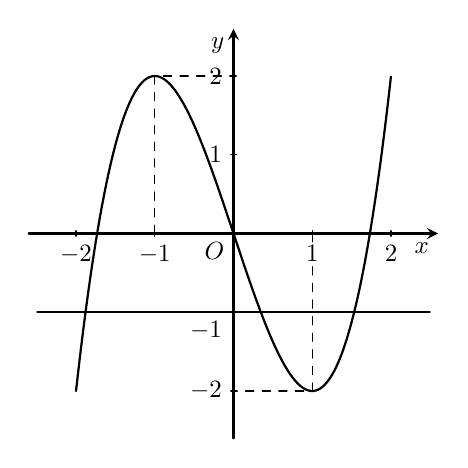
\begin{tikzpicture}[line join=round, line cap=round,>=stealth,thick]
				\tikzset{every node/.style={scale=0.9}}
				\draw[->] (-2.6,0)--(2.6,0) node[below left] {$x$};
				\draw[->] (0,-2.6)--(0,2.6) node[below left] {$y$};
				\draw (0,0) node [below left] {$O$};
				\foreach \x/\nx in {-2/-2,-1/-1,1/1,2/2}
				\draw[thin] (\x,1pt)--(\x,-1pt) node [below] {$\nx$};
				\foreach \y/\ny in {-2/-2,1/1,2/2}
				\draw[thin] (1pt,\y)--(-1pt,\y) node [left] {$\ny$};
				\foreach \z/\nz in {-1/-1}
				\draw[thin] (1pt,\z)--(-1pt,\z) node [below left] {$\nz$};
				\draw[dashed,thin](-1,0)--(-1,2)--(0,2);
				\draw[dashed,thin](1,0)--(1,-2)--(0,-2);
				\begin{scope}
					\clip (-2.5,-2.5) rectangle (2.5,2.5);
					\draw[samples=200,domain=-2:2,smooth,variable=\x] plot (\x,{1*((\x)^3)+0*((\x)^2)+-3*(\x)+0});
					\draw[samples=200,domain=-2.6:2.6,smooth,variable=\x] plot (\x,{-1});
				\end{scope}
			\end{tikzpicture}
		\end{center}
		Từ hình vẽ suy ra phương trình $f(x)=-1$ có $3$ nghiệm.
	}
\end{ex}
\begin{ex}%[Câu 5]%[2D1V5-3]
	Tìm tất cả các giá trị thực của tham số $m$ để đồ thị hàm số $y=x^3-3x^2$ cắt đường thẳng $y=m$ tại ba điểm phân biệt.
	\choice
	{$m\in (-\infty;-4 )$}
	{\True $m\in (-4;0 )$}
	{$m\in (0;+\infty)$}
	{$m\in (-\infty;-4 )\cup (0;+\infty)$}
	\loigiai{
		Ta có $y=x^3-3x^2 \Rightarrow y'=3x^2-6x;~y'=0 \Leftrightarrow \hoac{& x=0 \\& x=2}$\\
		Bảng biến thiên:\\
		\begin{center}
			
\begin{tikzpicture}
				\tkzTabInit[espcl=2.5,lgt=1.5]
				{$x$/0.7,$y'$/0.7,$y$/2.1}
				{$-\infty$,$0$,$2$,$+\infty$}
				\tkzTabLine{,+,0,-,0,+,}
				\tkzTabVar{-/$-\infty$,+/$0$,-/$-4$,+/$+\infty$}
			\end{tikzpicture}
		\end{center}
		Dựa vào bảng biến thiên ta thấy đồ thị hàm số $y=x^3-3x^2$ cắt đường thẳng $y=m$ tại ba điểm phân biệt khi $-4<m<0$.
	}
\end{ex}
\begin{ex}%[Câu 6]%[2D1N5-4]
	Đồ thị của hàm số $y=x^3-3x+2$ cắt trục tung tại điểm có tung độ bằng
	\choice
	{$0$}
	{$1$}
	{\True $2$}
	{$-2$}
	\loigiai{
	Ta có $f(0)=2$. Vậy đồ thị hàm số cắt trục tung tại điểm có tung độ bằng $2$.
	}
\end{ex}
\begin{ex}%[Câu 7]%[2D1H5-4]
	Số giao điểm của đồ thị hàm số $y=x^3+3x^2$ và đồ thị hàm số $y=3x^2+3x$ là
	\choice
	{\True $3$}
	{$1$}
	{$2$}
	{$0$}
	\loigiai{
		Phương trình hoành độ giao điểm của hai đồ thị đã cho là\\
		$x^3+3x^2=3x^2+3x \Leftrightarrow x^3-3x=0 \Leftrightarrow \hoac{& x=0 \\& x=\sqrt {3}\\& x=-\sqrt {3}.}\\$
		Hai đồ thị đã cho cắt nhau tại $3$ điểm.
	}
\end{ex}
\begin{ex}%[Câu 8]%[2D1N5-5]
	Cho hàm số $y=f(x)$ liên tục và xác định trên $\mathbb{R}.$ Biết $f(x)$ có đạo hàm $f'(x)$ và hàm số  $y=f'(x)$ có đồ thị như hình vẽ, khẳng định nào sau đây đúng?
	\begin{center}
		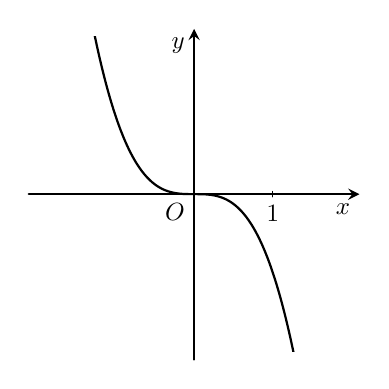
\begin{tikzpicture}[line join=round, line cap=round,>=stealth,thick]
			\tikzset{every node/.style={scale=0.9}}
			\draw[->] (-2.1,0)--(2.1,0) node[below left] {$x$};
			\draw[->] (0,-2.1)--(0,2.1) node[below left] {$y$};
			\draw (0,0) node [below left] {$O$};
			\foreach \x/\nx in {1/1}
			\draw[thin] (\x,1pt)--(\x,-1pt) node [below] {$\nx$};
			\begin{scope}
				\clip (-2,-2) rectangle (2,2);
				\draw[samples=200,domain=-2:2,smooth,variable=\x] plot (\x,{-1*((\x)^3)});
			\end{scope}
		\end{tikzpicture}
	\end{center}
	\choice
	{Hàm số $f(x)$ đồng biến trên $\mathbb{R}$
	}
	{Hàm số $f(x)$ nghịch biến trên $\mathbb{R}$}
	{Hàm số $f(x)$ nghịch biến trên $(-\infty;0)$}
	{\True Hàm số $f(x)$  nghịch biến trên $(0;+\infty)$}
	\loigiai{
		Trong khoảng $(0;+\infty)$ đồ thị hàm số $y=f'(x)$ nằm phía dưới trục hoành nên hàm số $f(x)$ nghịch biến trên khoảng $(0;+\infty)$.
	}
\end{ex}
\begin{ex}%[Câu 9]%[2D1H5-5]
	Cho hàm số $y=f(x)$ liên tục và xác định trên $[-2;2]$, có đồ thị của hàm số  $y=f'(x)$  như hình vẽ. Tìm giá trị $x_0$ để hàm số $y=f(x)$ đạt giá trị lớn nhất trên đoạn $[-2;2]$.
	\begin{center}
		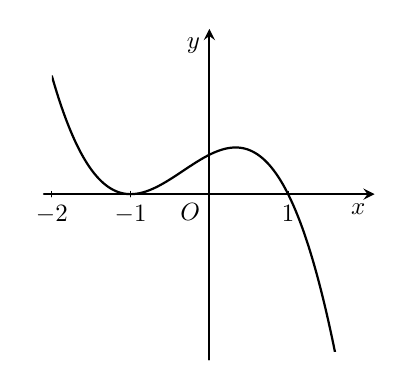
\begin{tikzpicture}[line join=round, line cap=round,>=stealth,thick]
			\tikzset{every node/.style={scale=0.9}}
			\draw[->] (-2.1,0)--(2.1,0) node[below left] {$x$};
			\draw[->] (0,-2.1)--(0,2.1) node[below left] {$y$};
			\draw (0,0) node [below left] {$O$};
			\foreach \x/\nx in {-2/-2,-1/-1,1/1}
			\draw[thin] (\x,1pt)--(\x,-1pt) node [below] {$\nx$};
			\begin{scope}
				\clip (-2,-2) rectangle (2,2);
				\draw[samples=200,domain=-2:2,smooth,variable=\x] plot (\x,{-0.5*((\x)^3)-0.5*((\x)^2)+0.5*(\x)+0.5});
			\end{scope}
		\end{tikzpicture}
	\end{center}
	\choice
	{$x_0=2$}
	{$x_0=-1$}
	{$x_0=-2$}
	{\True $x_0=1$}
	\loigiai{
		Từ đồ thị ta có bảng biến thiên
		\begin{center}
			
\begin{tikzpicture}
				\tkzTabInit[espcl=2.5,lgt=1.5]
				{$x$/0.7,$y'$/0.7,$y$/2.1}
				{$-2$,$-1$,$1$,$2$}
				\tkzTabLine{,+,0,+,0,-,}
				\tkzTabVar{-/,R,+/$f(1)$,-/}
			\end{tikzpicture}
		\end{center}
	}
\end{ex}
%Phương trình tiếp tuyến của đồ thị hàm số NB
\begin{ex}%[Câu 10]%[2D1N5-6]
	Đạo hàm của hàm số $y= f(x)$ tại điểm $x_0$ là hệ số góc của tiếp tuyến với đồ thị $(C)$ của hàm số tại điểm $M_0(x_0; f(x_0) )$. Khi đó phương trình tiếp tuyến của $(C)$ tại điểm $M_0$ là
	\choice
	{$y+y_0=f'(x_0)\cdot (x-x_0)$}
	{$y-y_0=f'(x_0)\cdot (x+x_0)$}
	{\True $y-y_0=f'(x_0)\cdot (x-x_0)$}
	{$y-y_0=f'(x_0)\cdot (x_0-x)$}
	\loigiai{
		
	}
\end{ex}
\begin{ex}%[Câu 11]%[2D1H5-6]
	Cho hàm số $y= x^3-2x+ 1.$ Viết phương trình tiếp tuyến của đồ thị hàm số tại điểm $M(0;1)$.
	\choice
	{$ y=2x +3$}
	{\True $ y=-2x + 1$}
	{$ y=4x + 1$}
	{$ y=-4x + 1$}
	\loigiai{
		Đạo hàm của hàm số đã cho là $y'= 3x^2-2$ $\Rightarrow$ $y'(0)=-2$.\\
		Phương trình tiếp tuyến của đồ thị hàm số tại điểm $M(0;1)$ là\\
		$y-1= -2(x-0)$ hay $ y=-2x + 1$.
	}
\end{ex}
\begin{ex}%[Câu 12]%[2D1V5-7]
	Đồ thị của hàm số $y=x^3-3mx^2-x+3m$ với $m$ là tham số đi qua bao nhiêu điểm cố định? 
	\choice
	{$1$}
	{\True $2$}
	{$3$}
	{$4$}
	\loigiai{
		Ta có $y=x^3-3mx^2-x+3m \Leftrightarrow (3x^2-3)m+y-x^3+x=0.$\\
		Phương trình nghiệm đúng với mọi $m$ khi $\heva{& 3x^2-3=0 \\& y-x^3+x=0.}\\$ 
		$\Leftrightarrow \hoac{& \heva{& x=1 \\& y=0}\\ & \heva{& x=-1\\& y=0.}\\}$ \\
		Đồ thị hàm số có hai điểm cố định.
	}
\end{ex}

\cauds
\begin{ex}%[Câu 1]
	Cho một hàm số có đồ thị như sau
	\begin{center}
		\begin{tikzpicture}[line join=round, line cap=round,>=stealth,thick]
			\tikzset{every node/.style={scale=0.9}}
			\draw[->] (-3.1,0)--(4.1,0) node[below left] {$x$};
			\draw[->] (0,-3.1)--(0,4.1) node[below left] {$y$};
			\draw (0,0) node [below left] {$O$};
			\foreach \x/\nx in {1/1,-1/-1}
			\draw[thin] (\x,1pt)--(\x,-1pt) node [below left] {$\nx$};
			\foreach \y/\ny in {1/1,-1/-1}
			\draw[thin] (1pt,\y)--(-1pt,\y) node [below left] {$\ny$};
			\draw[dashed,thin] (1.01,-3)--(1.01,4);
			\begin{scope}
				\clip (-3,-3) rectangle (4,4);
				\draw[samples=200,domain=-3:0.99,smooth,variable=\x] plot (\x,{(1*(\x)+1)/(1*(\x)+-1)});
				\draw[samples=200,domain=1.01:4,smooth,variable=\x] plot (\x,{(1*(\x)+1)/(1*(\x)+-1)});
				\draw[dashed,thin] (-3,1/1)--(4,1/1);
			\end{scope}
		\end{tikzpicture}
	\end{center}
	\choiceTF
	{Đây là đồ thị của một hàm số đồng biến}
	{\True Đồ thị có tiệm cận đứng là $x=1$}
	{Đồ thị có tiệm cận ngang là $y=0$}
	{\True Đường cong trên là đồ thị của hàm số $y=\dfrac{x+1}{x-1}$}
	\loigiai{
		\begin{itemchoice}
			\itemch Sai vì nhìn từ trái sang phải đồ thị hướng xuống nên hàm số nghịch biến.
			\itemch Đúng.
			\itemch Sai vì nhìn vào đồ thị ta thấy tiệm cận ngang là $y=1.$
			\itemch Đúng.
		\end{itemchoice}
	}
\end{ex}

\begin{ex}%[Câu 2]
	Cho hàm số $f( x)=a{{x}^{4}}+b{{x}^{2}}+c$ có đồ thị là đường cong trong hình bên.
	\begin{center}
		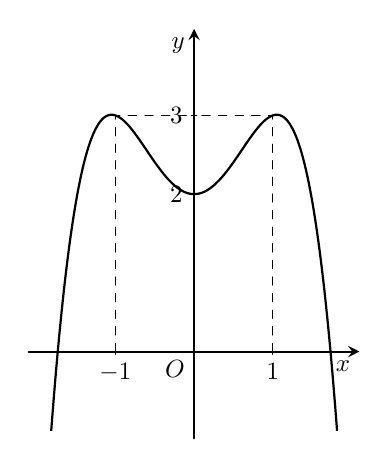
\begin{tikzpicture}[line join=round, line cap=round,>=stealth,thick]
			\tikzset{every node/.style={scale=0.9}}
			\draw[->] (-2.1,0)--(2.1,0) node[below left] {$x$};
			\draw[->] (0,-1.1)--(0,4.1) node[below left] {$y$};
			\draw (0,0) node [below left] {$O$};
			\foreach \x/\nx in {-1/-1,1/1}
			\draw[thin] (\x,1pt)--(\x,-1pt) node [below] {$\nx$};
			\foreach \y/\ny in {2/2,3/3}
			\draw[thin] (1pt,\y)--(-1pt,\y) node [left] {$\ny$};
			\draw[dashed,thin](-1,0)--(-1,3)--(0,3);
			\draw[dashed,thin](1,0)--(1,3)--(0,3);
			\begin{scope}
				\clip (-2,-1) rectangle (2,4);
				\draw[samples=200,domain=-2:2,smooth,variable=\x] plot (\x,{-5/6*((\x)^4)+0*((\x)^3)+11/6*((\x)^2)+0*(\x)+2});
			\end{scope}
		\end{tikzpicture}
	\end{center}
	\choiceTF
	{\True Đồ thị của hàm số cắt trục hoành tại 2 điểm phân biệt}
	{\True Số nghiệm thực của phương trình $f\left( x \right)=1$ là 2}
	{Số nghiệm thực của phương trình $f\left( x \right)=\dfrac{3}{2}$ là 3}
	{\True Phương trình $f\left( x \right)-3=0$ có tổng các nghiệm bằng 0}
	\loigiai{
		\begin{itemchoice}
			\itemch Đúng.
			\itemch Đúng vì đường thẳng $y=1$ cắt đồ thị tại 2 điểm nên $f\left( x \right)=1$ có 2 nghiệm.
			\itemch Sai vì đường thẳng $y=\dfrac{3}{2}$ cắt đồ thị tại 2 điểm nên $f\left( x \right)=\dfrac{3}{2}$ có 2 nghiệm.
			\itemch Đúng vì đường thẳng $y=3$ cắt đồ thị tại 2 điểm ${{x}_{1}}=-1,{{x}_{2}}=1$  nên $f\left( x \right)-3=0$ có tổng các nghiệm bằng 0.
		\end{itemchoice}
	}
\end{ex}

\begin{ex}%[Câu 3]
	Hàm số $y=f\left( x \right)$ liên tục trên khoảng $K$, biết đồ thị của hàm số $y=f'\left( x \right)$ trên $K$ như hình vẽ bên dưới.
	\begin{center}
		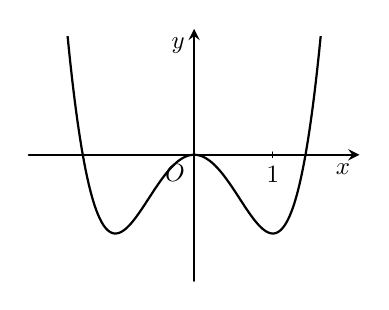
\begin{tikzpicture}[line join=round, line cap=round,>=stealth,thick]
			\tikzset{every node/.style={scale=0.9}}
			\draw[->] (-2.1,0)--(2.1,0) node[below left] {$x$};
			\draw[->] (0,-1.6)--(0,1.6) node[below left] {$y$};
			\draw (0,0) node [below left] {$O$};
			\foreach \x/\nx in {1/1}
			\draw[thin] (\x,1pt)--(\x,-1pt) node [below] {$\nx$};
			\begin{scope}
				\clip (-2,-1.5) rectangle (2,1.5);
				\draw[samples=200,domain=-2:2,smooth,variable=\x] plot (\x,{1*((\x)^4)+0*((\x)^3)+-2*((\x)^2)+0*(\x)+0});
			\end{scope}
		\end{tikzpicture}
	\end{center}
	\choiceTF
	{Đồ thị của hàm số $y=f'\left( x \right)$ cắt trục hoành tại 3 điểm phân biệt}
	{Hàm số $y=f\left( x \right)$ đồng biến trên khoảng $\left( 0;1 \right)$}
	{Hàm số $y=f\left( x \right)$ nghịch biến trên khoảng $\left( -1;1 \right)$}
	{Hàm số $y=f\left( x \right)$ có 2 cực trị}
	\loigiai{
		\begin{itemchoice}
			\itemch Đúng.
			\itemch Sai vì trong khoảng $\left( 0;1 \right)$ đồ thị nằm phía dưới trục $Ox$.
			\itemch Đúng vì trong khoảng $\left( -1;1 \right)$ đồ thị nằm phía dưới trục $Ox$.
			\itemch Đúng.
		\end{itemchoice}
	}
\end{ex}

\begin{ex}%[Câu 4]
	Cho đường cong  $(C):y={{x}^{3}}-4$
	\choiceTF
	{Hệ số góc của tiếp tuyến với đường cong $\left( C \right)$ tại điểm $M\left( 0;-4 \right)$ là $1$}
	{Phương trình tiếp tuyến của đường cong $\left( C \right)$ tại điểm có hoành độ bằng $1$ là $y=3x-9$}
	{\True Phương trình tiếp tuyến của đường cong $\left( C \right)$ tại điểm có tung độ bằng $4$ là $y=12x-20$}
	{\True Phương trình tiếp tuyến của đường cong $\left( C \right)$ đi qua điểm $A\left( 2;4 \right)$ là $y=3x-2$ và $y=12x-20$}
	\loigiai{
		\begin{itemchoice}
			\itemch Sai vì hệ số góc tại điểm $M\left( 0;-4 \right)$ là $y'\left( 0 \right)={{3.0}^{2}}=0$.
			\itemch Sai vì ta có $y'=3{{x}^{2}}\Rightarrow y'\left( 1 \right)=3.$ Phương trình tiếp tuyến: $y=3.\left( x-1 \right)-3=3x-9$
			\itemch Đúng vì tung độ bằng 4 suy ra hoành độ bằng 2.\\
			$y'=3{{x}^{2}}\Rightarrow y'\left( 2 \right)=12.$ Phương trình tiếp tuyến $y=12.\left( x-2 \right)+4=12x-20.$
			\itemch Đúng vì ta có $y'=3{{x}^{2}}$. Gọi $M\left( {{x}_{0}};{{y}_{0}} \right)$ là tọa độ tiếp điểm.\\
			Phương trình tiếp tuyến của $\left( C \right)$ tại điểm $M$ có dạng $y=3{{x}_{0}}^{2}.\left( x-{{x}_{0}} \right)+{{x}_{0}}^{3}-4$.\\
			Vì tiếp tuyến đi qua điểm $A\left( 2;4 \right)$  nên ta có\\
			$4=3{{x}_{0}}^{2}\left( 2-{{x}_{0}} \right)+{{x}_{0}}^{3}-4\Leftrightarrow -2{{x}_{0}}^{3}+6{{x}_{0}}^{2}-8=0\Leftrightarrow x_{0}=-1,x_{0}=2$.\\
			Với ${{x}_{0}}=-1$ suy ra phương trình tiếp tuyến là $y=3x-2.$\\
			Với ${{x}_{0}}=2$ suy ra phương trình tiếp tuyến là $y=12x-20.$
		\end{itemchoice}
	}
\end{ex}

\caukq
\begin{ex}%[2D1H5-1]
	Cho hàm số $y=\dfrac{ax+2}{bx-2}$ với $a,b\in \mathbb{Z}$ có đồ thị như hình bên dưới. Tính giá trị của biểu thức $T=a+b$.
	\begin{center}
		\begin{tikzpicture}[line join=round, line cap=round,>=stealth,thick]
			\tikzset{every node/.style={scale=0.9}}
			\draw[->] (-2.6,0)--(6.1,0) node[below left] {$x$};
			\draw[->] (0,-2.1)--(0,6.1) node[below left] {$y$};
			\draw (0,0) node [below left] {$O$};
			\foreach \x/\nx in {-2/-2,2/2}
			\draw[thin] (\x,1pt)--(\x,-1pt) node [below] {$\nx$};
			\foreach \y/\ny in {-1/-1,1/1}
			\draw[thin] (1pt,\y)--(-1pt,\y) node [left] {$\ny$};
			\draw[dashed,thin] (2.01,-2)--(2.01,6);
			\draw[dashed,thin] (2.01,-2)--(2.01,6);
			\begin{scope}
				\clip (-2.5,-2) rectangle (6,6);
				\draw[samples=200,domain=-2.5:1.99,smooth,variable=\x] plot (\x,{(1*(\x)+2)/(1*(\x)+-2)});
				\draw[samples=200,domain=2.01:8,smooth,variable=\x] plot (\x,{(1*(\x)+2)/(1*(\x)+-2)});
				\draw[dashed,thin] (-2.5,1/1)--(8,1/1);
			\end{scope}
		\end{tikzpicture}
	\end{center}
	\shortans[0]{2}
	\loigiai{
		Đường tiệm cận đứng là $x=2$ thì $\dfrac{2}{b}=2\Rightarrow b=1$.\\
		Đường tiệm cận ngang là $y=1$ thì $\dfrac{a}{1}=1\Rightarrow a=1$.\\
		Vậy $T=a+b=1+1=2$.
	}
\end{ex}
\begin{ex}%[2D1N5-4]
	Biết đường thẳng $y=-2x+2$ cắt đồ thị hàm số $y=x^{3}+x+2$ tại điểm duy nhất có tọa độ là $\left ( x_{0} ;y_{0}\right )$. Tính giá trị của biểu thức $T=x_{0}-y_{0}$.
	\shortans[0]{$-2$}
	\loigiai{
		Phương trình hoành độ giao điểm là $-2x+2=x^{3}+x+2\Leftrightarrow x^{3}+3x=0\Leftrightarrow x=0\Rightarrow y=2$. \\
		Vậy tọa độ giao điểm là $\left ( 0;2 \right )$ \\
		Khi đó, $T=0-2=-2$.
	}
\end{ex}
\begin{ex}%[2D1V5-5]
	Cho hàm số $y=f\left ( x \right )$ liên tục trên $\mathbb{R}$ và hàm số $y=f'\left ( x \right )$ có đồ thị như hình vẽ.
	\begin{center}
		\begin{tikzpicture}[line join=round, line cap=round,>=stealth,thick]
			\tikzset{every node/.style={scale=0.9}}
			\draw[->] (-1.1,0)--(6.1,0) node[below left] {$x$};
			\draw[->] (0,-1.1)--(0,6.1) node[below left] {$y$};
			\draw (0,0) node [below left] {$O$};
			\foreach \x/\nx in {1/x_1,3/x_2,4/x_3}
			\draw[thin] (\x,1pt)--(\x,-1pt) node [below] {$\nx$};
			\foreach \y/\ny in {1/1,2/2,5/5}
			\draw[thin] (1pt,\y)--(-1pt,\y) node [left] {$\ny$};
			\draw[dashed,thin](1,0)--(1,5)--(0,5);
			\draw[dashed,thin](3,0)--(3,1)--(0,1);
			\draw[dashed,thin](4,0)--(4,2)--(0,2);
			\begin{scope}
				\clip (-1,-1) rectangle (6,6);
				\draw[name path=] plot[smooth,tension=0.7] coordinates{(-1,-2)(1,5)(3,1)(4,2)(5,-1)};
			\end{scope}
		\end{tikzpicture}
	\end{center}
	Hàm số $y=f\left ( x \right )+\dfrac{2017-2018x}{2017}$ có bao nhiêu điểm cực trị?
	\shortans[0]{4}
	\loigiai{
		Ta có $y'=f'(x)=\dfrac{2018}{2017}$.\\
		Khi đó, $y'=0\Leftrightarrow f'\left ( x \right )-\dfrac{2018}{2017}=0\Leftrightarrow f'\left ( x \right )=\dfrac{2018}{2017}$.\\
		Dựa vào đồ thị, ta thấy phương trình $f'(x)=\dfrac{2018}{2017}$ có 4 nghiệm phân biệt. Do đó, hàm số đã cho có 4 điểm cực trị.
	}
\end{ex}
\begin{ex}%[2D1V5-6]
	Cho hàm số $y=\dfrac{1}{3}x^{3}-2x^{2}+3x+5$. Biết phương trình tiếp tuyến của đồ thị hàm số với hệ số góc nhỏ nhất có dạng là $y=ax+b \left ( a,b\in \mathbb{R} \right )$. Tính giá trị của biểu thức $T=a+3b$.
	\shortans[0]{}
	\loigiai{
		Ta có: $y'=x^{2}-4x+3$.\\
		Khi đó, $\min y'=y'\left ( 2 \right )=-1\Rightarrow x^{2}-4x+3=-1\Rightarrow x=2\Rightarrow y=\dfrac{17}{3}$.\\
		Phương trình tiếp tuyến là $y=-1\left ( x-2 \right )+\dfrac{17}{3}=-x+\dfrac{23}{3}$. \\
		Vậy $T=-1+3.\dfrac{23}{3}=22$.
	}
\end{ex}
\begin{ex}%[2D1C5-3]
	Cho hàm số $y=f\left ( x \right )$ liên tục trên $\left [ 1;3 \right ]$ và có bảng biến thiên như sau
	\begin{center}
		
\begin{tikzpicture}
			\tkzTabInit[espcl=2.5,lgt=1.5]
			{$x$/0.7,$f'(x)$/0.7,$f(x)$/2.1}
			{$1$,$2$,$3$}
			\tkzTabLine{,+,0,-,}
			\tkzTabVar{-/$1$,+/$4$,-/$3$}
		\end{tikzpicture}
	\end{center}
	Có bao nhiêu giá trị nguyên của $m$ để phương trình $f\left ( x+1 \right )=\dfrac{m}{x^{2}-4x+5}$ có nghiệm trên khoảng $\left ( 1;2 \right )$?
	\shortans[0]{4}
	\loigiai{
		Ta có: $y'=x^{2}-4x+3$.\\
		Vì $x^{2}-4x+5=\left ( x-2 \right )^{2}+1>0, \forall x\in \mathbb{R}$ nên $f\left ( x+1 \right )=\dfrac{m}{x^{2}-4x+5}\Leftrightarrow \left ( x^{2}-4x+5 \right )f\left ( x+1 \right )=m$.\\
		Đặt $h\left ( x \right )=\left ( x^{2}-4x+5 \right )f\left ( x+1 \right )$ với $x\in \left ( 1;2 \right )$. \\
		Ta có $h'\left ( x \right )=\left ( x^{2}-4x+5 \right )f'\left ( x+1 \right )+\left ( 2x-4 \right )f\left ( x+1 \right )$. \\
		Dựa vào bảng biến thiên của hàm số $y=f\left ( x \right )$, ta có $\forall x\in \left ( 1;2 \right )\Rightarrow x+1\in \left ( 2;3 \right )\Rightarrow f'\left ( x+1 \right )\leqslant 0$ và $2x-4<0,\forall x\in \left ( 1;2 \right );f\left ( x+1 \right )\geqslant 3>0,x+1\in \left ( 2;3 \right )$. \\
		Do đó, $h'\left ( x \right )<0,\forall x\in \left ( 1;2 \right )$. \\
		Bảng biến thiên của hàm số $h\left ( x \right )$ trên khoảng $\left ( 1;2 \right )$ như sau
		\begin{center}
			
\begin{tikzpicture}
				\tkzTabInit[espcl=2.5,lgt=1.5]
				{$x$/0.7,$h'(x)$/0.7,$h(x)$/2.1}
				{$1$,$2$}
				\tkzTabLine{,-,}
				\tkzTabVar{+/$h(1)$,-/$h(2)$}
			\end{tikzpicture}
		\end{center}
		Khi đó, phương trình $h\left ( x \right )=m$ có nghiệm $x\in \left ( 1;2 \right )$ khi và chỉ khi $h\left ( 2 \right )<m<h\left ( 1 \right )$ \\
		$\Rightarrow 1.f\left ( 3 \right )<m<2.f\left ( 2 \right )\Leftrightarrow 3<m<8$. \\
		Vậy có 4 giá trị nguyên của $m$ thỏa mãn yêu cầu bài toán.
	}
\end{ex}
\begin{ex}%[2D1C5-7]
	Cho hàm số $y=\dfrac{2x-1}{x+1}$ có đồ thị (C). Tính tổng hoành độ của hai điểm nằm trên (C) đối xứng nhau qua đường thẳng $d:y=3x+5$.
	\shortans[0]{-2}
	\loigiai{
		Gọi $\Delta$ là đường thẳng vuông góc với $d$. Khi đó, $\Delta$ có dạng $y=-\dfrac{1}{3}x+a$.\\
		Phương trình hoành độ giao điểm của (C) và $\Delta$ là \\
		$\dfrac{2x-1}{x+1}=-\dfrac{1}{3}x+a\Leftrightarrow x^{2}+\left ( 7-3a \right )x-3-3a=0 \left ( x\neq -1 \right )$ (1). \\
		$\Delta$ cắt (C) tại 2 điểm phân biệt khi (1) có hai nghiệm phân biệt khác $-1$.\\
		$\left\{\begin{matrix}
			\Delta =\left ( 7-3a \right )^{2}+12\left ( 1+a \right )>0 &  \\
			1-\left ( 7-3a \right )-3-3a\neq 0 &  \\
		\end{matrix}\right.\Leftrightarrow 9a^{2}-30a+61>0$ (Đúng với mọi $a$).\\
		Khi đó, $\Delta$ cắt (C) tại hai điểm $A,B$ có hoành độ lần lượt là $x_{1},x_{2}$ là nghiệm của phương trình (1).\\
		Gọi $M$ là trung điểm của $AB$, ta có $M\left ( \dfrac{x_{1}+x_{2}}{2};-\dfrac{x_{1}+x_{2}}{6}+a\right )$ hay $M\left (\dfrac{3a-7}{2};\dfrac{3a+7}{6} \right )$. \\
		Mặt khác, $M\in d$ nên $\dfrac{3a+7}{6}=\dfrac{3\left ( 3a-7 \right )}{2}+5\Leftrightarrow a=\dfrac{5}{3}$.\\
		Khi đó, (1) trở thành $x^{2}+2x-8=0\Leftrightarrow x=2; x=-4$.\\
		Vậy tổng hoành độ hai điểm thỏa yêu cầu bằng $2+\left ( -4 \right )=-2$.
	}
\end{ex}